\renewcommand{\thechapter}{\Roman{chapter}}
\chapter{Methodology}
\renewcommand{\thechapter}{\arabic{chapter}}
\label{ch4:Methodology}
\thispagestyle{empty}

In this chapter, the study discusses the systematic approach employed in the development of of the proposed system. As depicted in Figure \ref{ch4:fig:system_development_process}, each phases is essential in shaping the overall system functionality. This chapter explains the approach taken, giving an overview of the techniques, methods, and resources applied at every development step.

\begin{figure}[H]
	\centering
	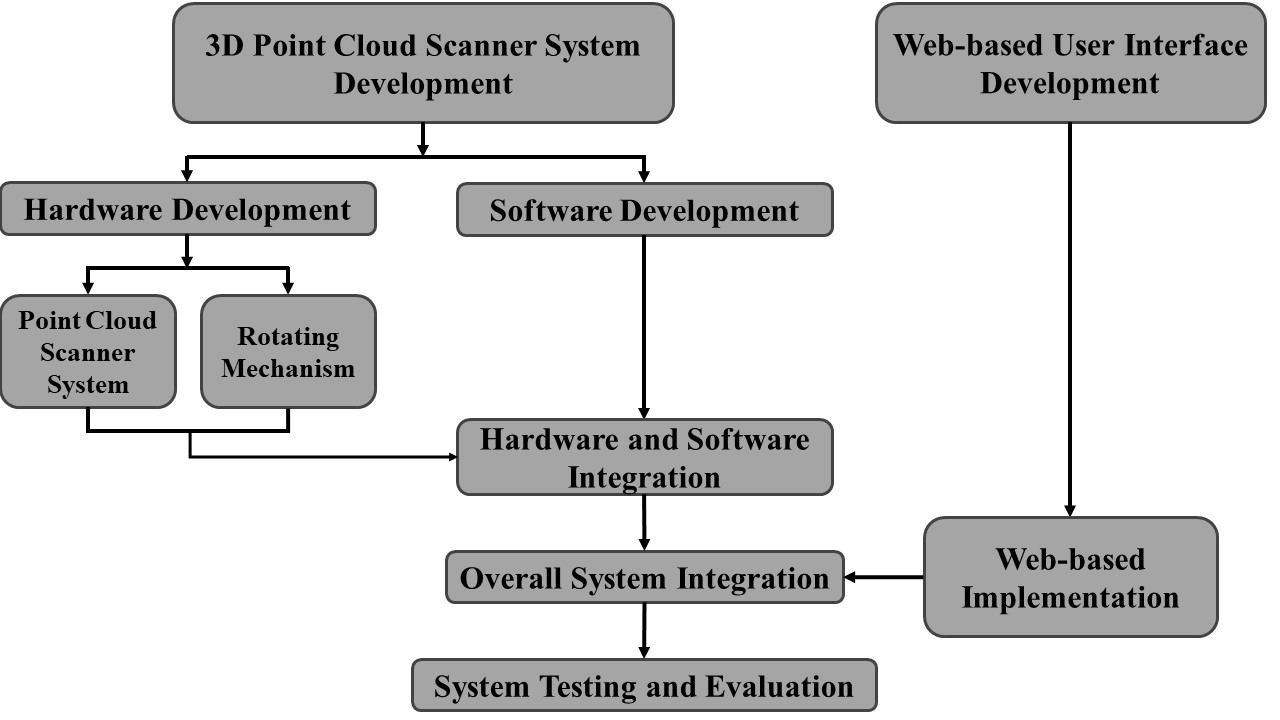
\includegraphics[width=1\textwidth]{Figures/system_development_process}
	\caption{System Development Process}
	\label{ch4:fig:system_development_process}
\end{figure}

\section{System Requirements Analysis}
\label{ch4:sec:system_requirements_analysis}

The development process of the study encompasses hardware, software, and web-based application design, followed by system integration and testing. As depicted in Figure \ref{ch4:fig:overall_system_setup_development} which is the proposed overall system setup, the study undertook the design and development of two distinct yet interconnected systems: the 3D Point Cloud Scanner (3D-PCSS), which is placed at the top of a storage bin, and the web-based application which is both connected to the local network. This overall system setup achieved by following a step by step development process which is illustrated in figure \ref{ch4:fig:system_development_process}, identifying hardware aspect which involves selecting and configuring the necessary components for data acquisition, processing, and communication. software development focuses on programming the processes to control hardware functionality and execute specific tasks. Meanwhile, web-based application design requires creating an interface for users to interact and data visualization. System integration involves bringing together these components and ensuring communication and functionality between them. Lastly, system testing and evaluation was conducted to validate the functionality, performance, and reliability of the developed systems through various testing procedures.

\begin{figure}[H]
	\centering
	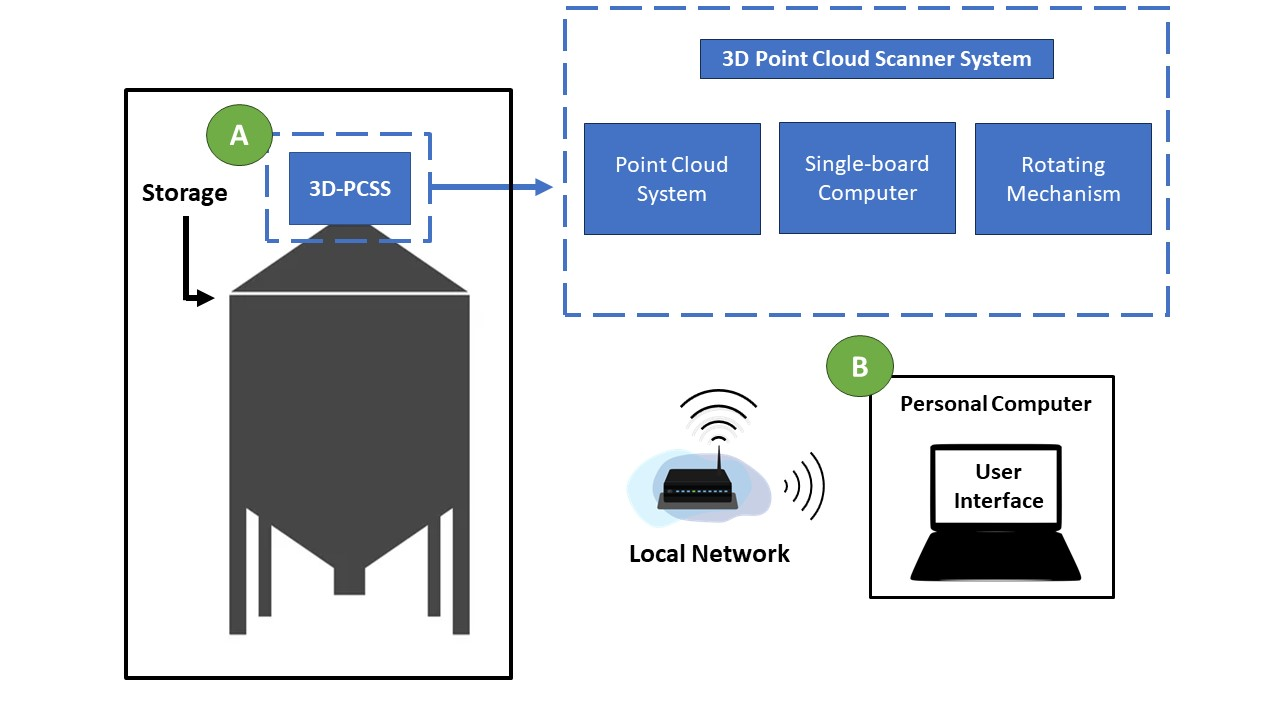
\includegraphics[width=1\textwidth]{Figures/system_analysis}
	\caption{Overall System Setup: (A) 3D-PCSS, (B) User Interface}
	\label{ch4:fig:overall_system_setup_development}
\end{figure}

\section{Hardware Development}
\label{ch4:sec:hardaware_design}

The hardware development conducted in this study involves the design and construction of 3D point cloud scanner and storage bin. The storage bin was created for testing and evaluation of the overall system.

% The researcher will adopt the concept of tilting method using a 2D of-the-shelf LiDAR to acquire 3D point cloud data to minimize the cost compared to commercial 3D LiDAR. The hardware and physical components of 3D point cloud scanner are composed of three major components, the 2D LiDAR device, the tilting mechanism which include the fabricated holder for mechanical tilting and the motor for the rotation movement. In Figure \ref{ch4:fig:System Hardware Block Diagram}, the 3D point cloud scanner is placed at the top of the flour bin.

% \begin{figure}
% 	\centering
% 	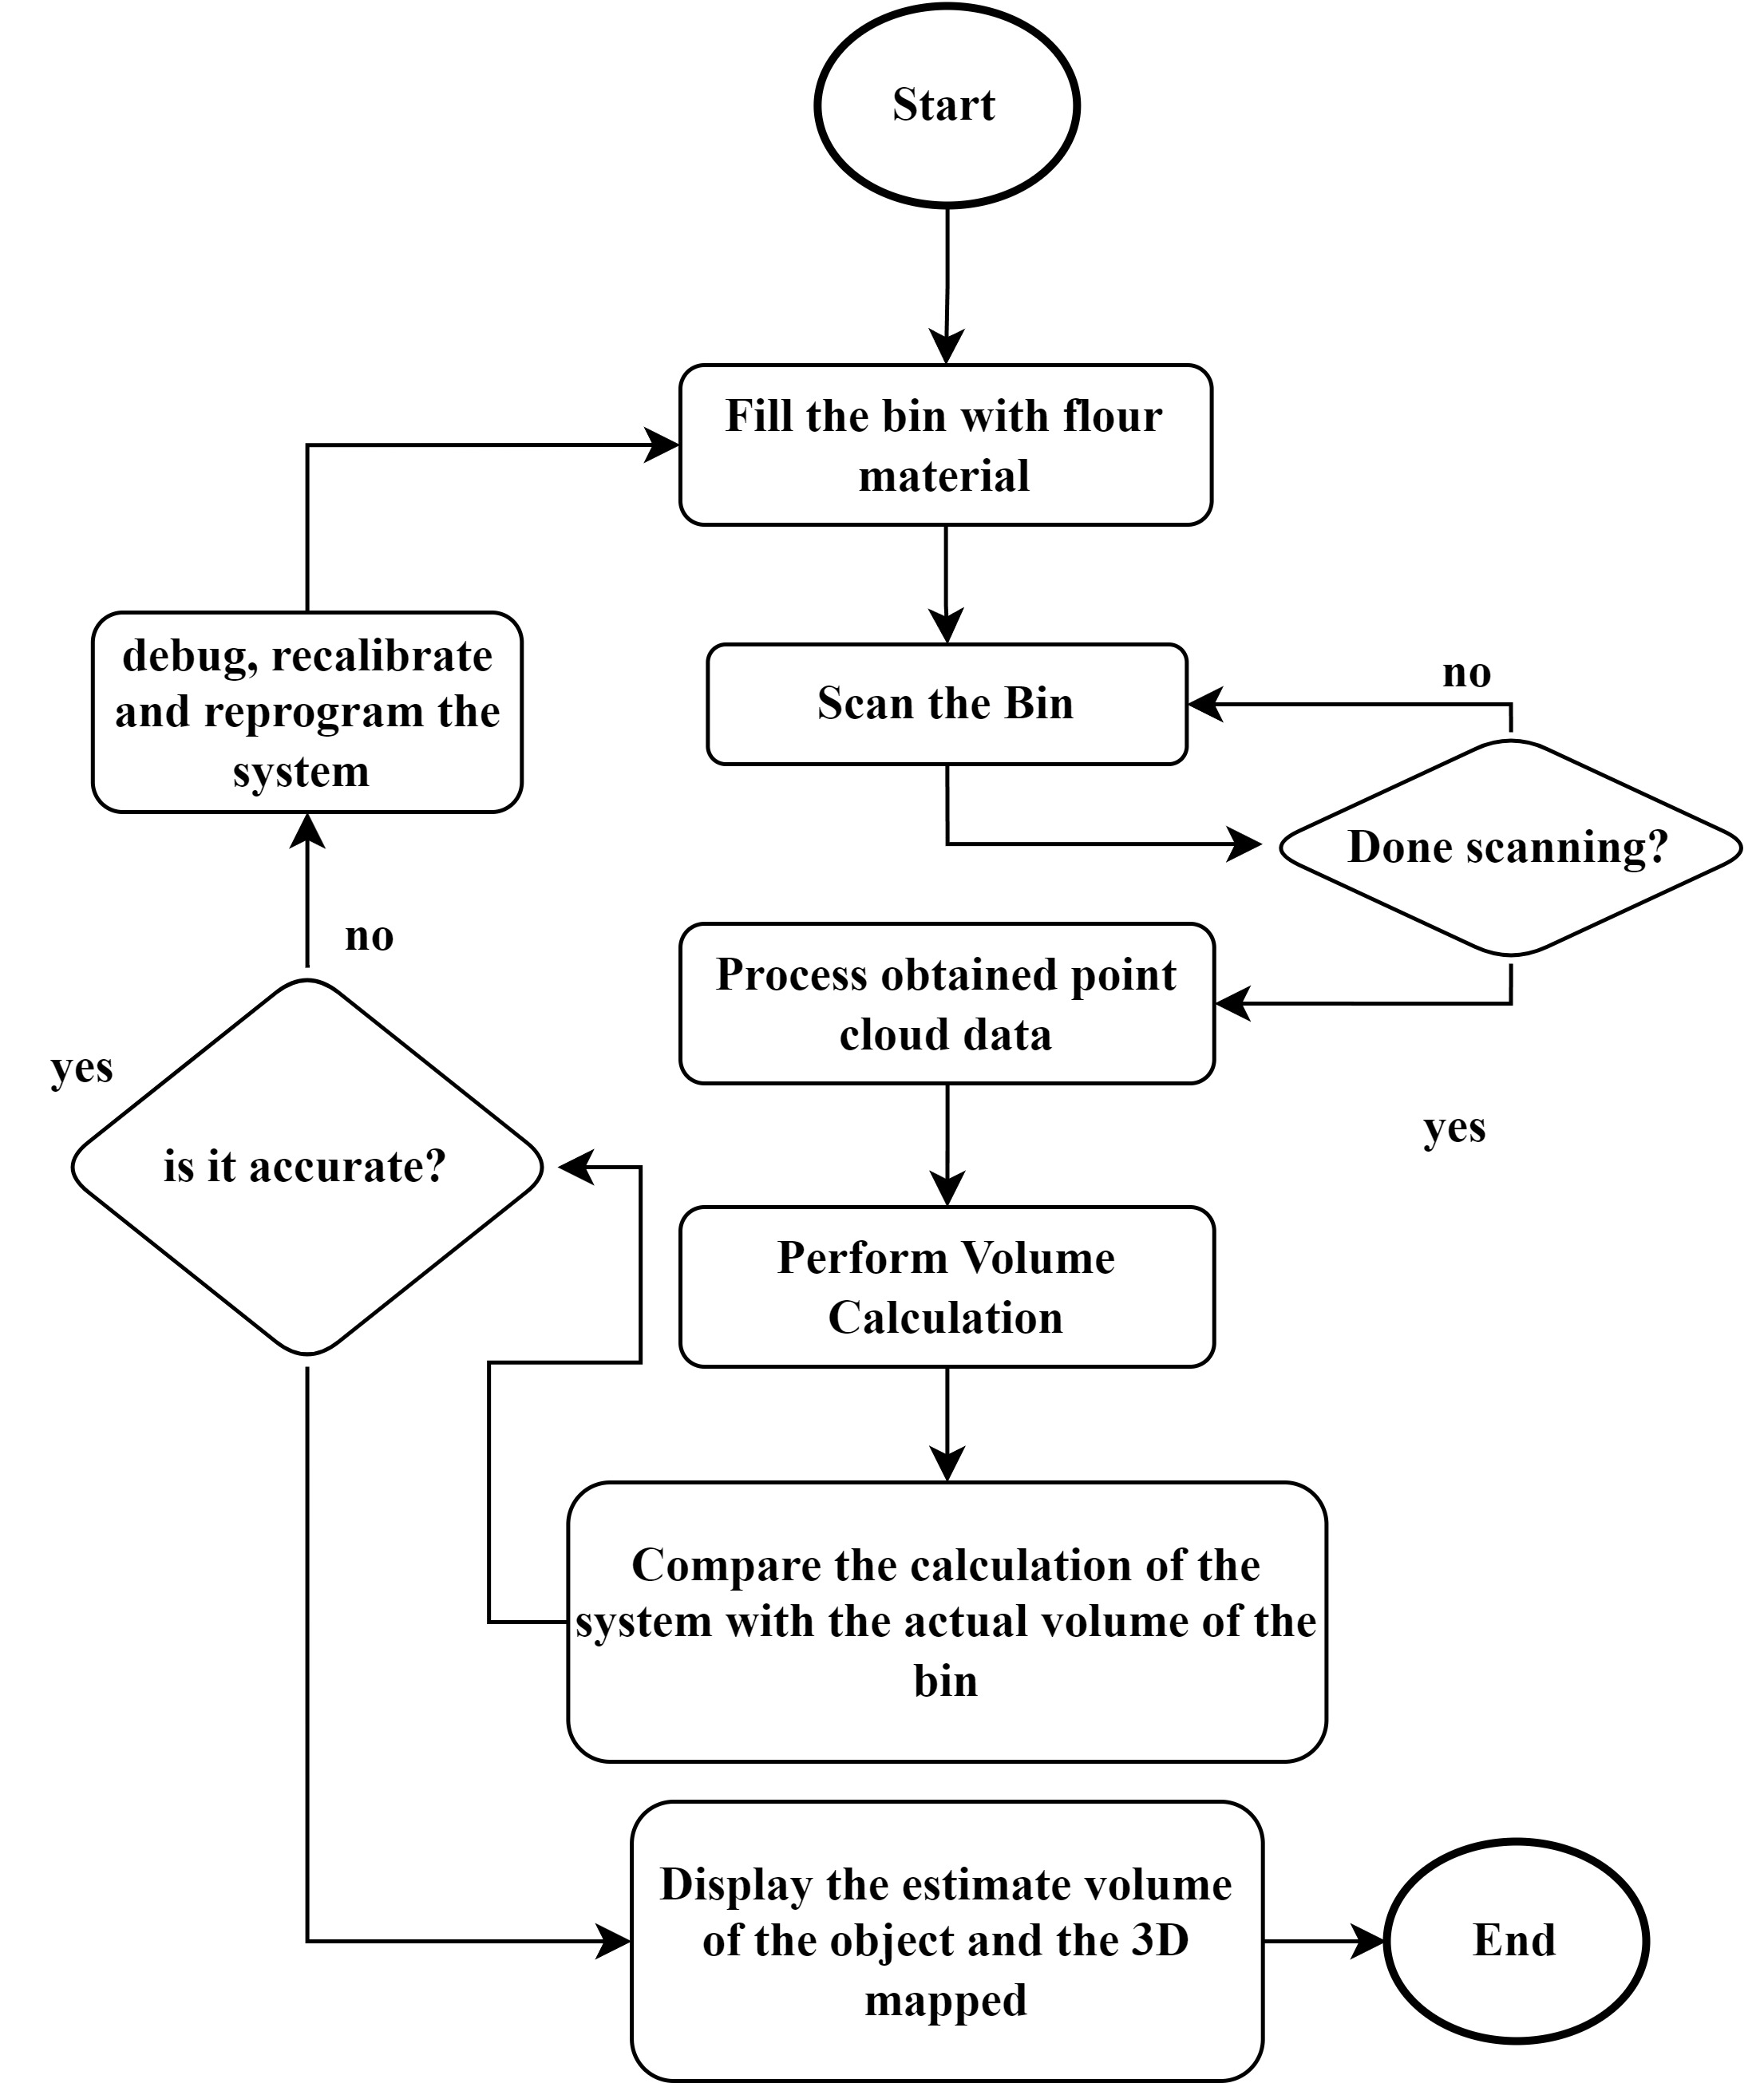
\includegraphics[width=0.9\textwidth]{Figures/general-flowchart-of-the-system-2.jpg}
% 	\caption{General Flowchart of the System}
% 	\label{ch4:fig:General flowchart of the system}
% \end{figure}

\subsection{Creating a Storage Bin}
\label{ch4:subsec:Modeling of Flour Bin}
The study involves constructing a mock-up flour storage bin modeled after those commonly used in food manufacturing industries. The mock-up bin is designed to closely mimic the geometric shape and proportions of real storage bins used in practice.

\subsection{3D Point Cloud Scanner Design (3D-PCSS)}
\label{ch4:subsec:3d_point_cloud_scanner_design}

\subsubsection*{Point Cloud Scanner System}

Point cloud devices, such as LiDAR (Light Detection and Ranging), offer exceptional accuracy in acquiring distance measurements over considerable distances. LiDAR systems emit laser pulses and measure the time it takes for these pulses to return after bouncing off objects in the environment. This technology enables the creation of highly detailed and accurate three-dimensional point clouds, which represent the surfaces and structures within the scanned area. Even low-cost LiDAR options are available in the market, making this technology accessible for various applications and budgets.

The point cloud scanner system in this study used a low-cost 2D LiDAR device controlled with single-board computer (SBC) for its computing functionality. \\

\subsubsection*{Rotating Mechanism}

The rotating mechanism design which is attached to the 2D LiDAR in this study is based on the methodology outlined in a previous research conducted by \citet{clar2022}. This prior study served as a foundational framework for the development of the rotating 2D LiDAR system in this study, providing into the integration of a pan-tilt unit (PTU) with a 2D LiDAR scanner to enable three-dimensional point cloud scanning. By employment the principles and techniques conducted in \citet{clar2022}, the current study aims to further refine and enhance the performance of the rotating 2D LiDAR system for its intended application and also address the problem encountered in the previous study.

The servo motor utilized in this study was the AX-12A Dynamixel, known for its high precision and reliability in robotic applications. What sets this servo apart is its compatibility with a Software Development Kit (SDK), which includes configurations for integration with the Robot Operating System (ROS). This feature enables communication and control of the servo motor within the ROS ecosystem, allowing for flexible and efficient development of robotic systems. This feature enables the LiDAR and Servo to communicate and synchronize, figure \ref{ch4:fig:servo_lidar_comm} shows the synchronization of the LiDAR and servo. \\

% \begin{algorithm}[]
% 	\caption{LDA}
% 	\label{ch4:algo:servo_and_lidar}
% 	\begin{algorithmic}[1]
% 		\FOR{$d$}
% 		\STATE{
% 			\FOR{$k\in\{1,...,K\}$}
% 			\STATE{Generate$\beta_k=(\beta_{k_1},...,\beta_{k,V})^T \sim Dirichlet(\cdot\vert\eta)$}
% 			\ENDFOR
% 		}
% 		\ENDFOR
% 	\end{algorithmic}
% \end{algorithm}

\begin{figure}[H]
	\centering
	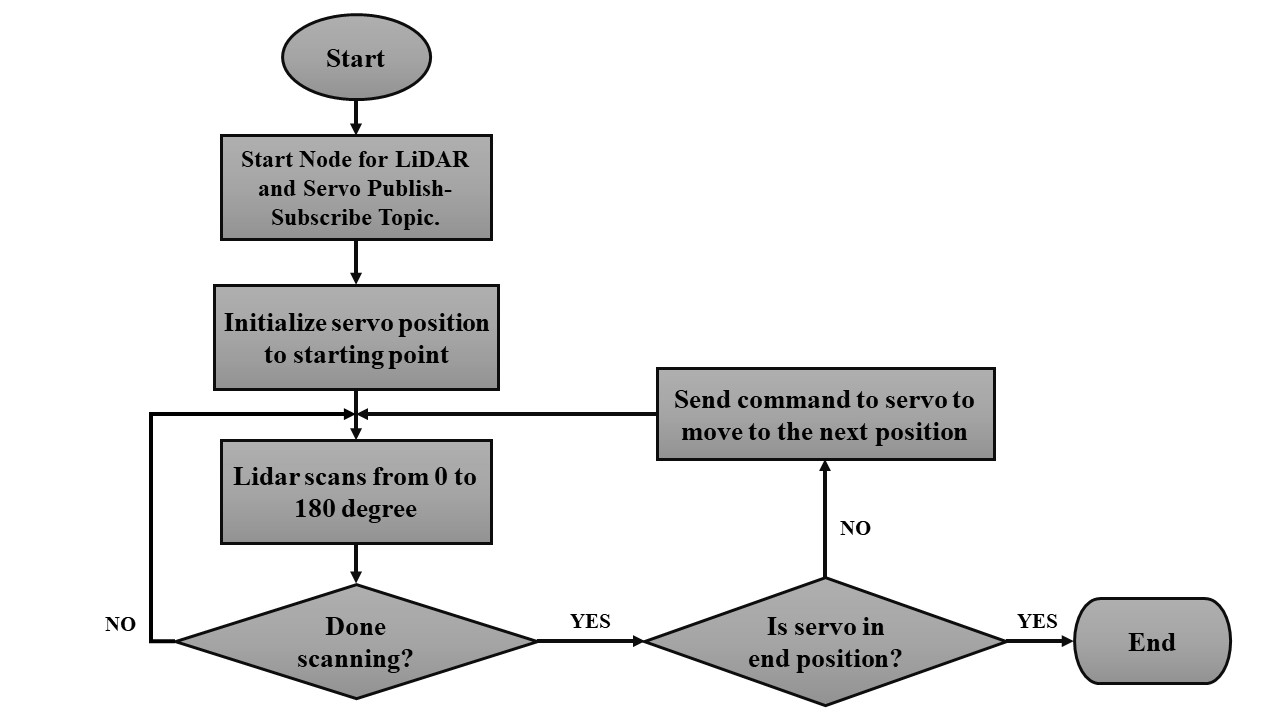
\includegraphics[width=1\textwidth]{Figures/servo_lidar_comm}
	\caption{Synchronization Process of LiDAR and Servo}
	\label{ch4:fig:servo_lidar_comm}
\end{figure}

The 3D-PCSS is the integration of point cloud scanner system and rotating mechanism. The major components of the system is illustrated in the figure \ref{ch4:fig:components_of_3d-pcss}, the hardware design flow chart of the system is shown in figure \ref{ch4:fig:3d-pcss_development_flow_chart}. The 3D-PCSS in this study considers the following design and functionality:
\begin{itemize}
	\item Based on low-cost 2D LiDAR device.
	\item Able to establish the communication between the rotating mechanism and LiDAR device.
	\item Able to gather and process 3D point cloud data.
	\item Support for connecting to a local network for remote data visualization and monitoring.
	\item Utilizing Robot Operating System (ROS) and Point Cloud Library (PCL) for its firmware development.
\end{itemize}

\begin{figure}[H]
	\centering
	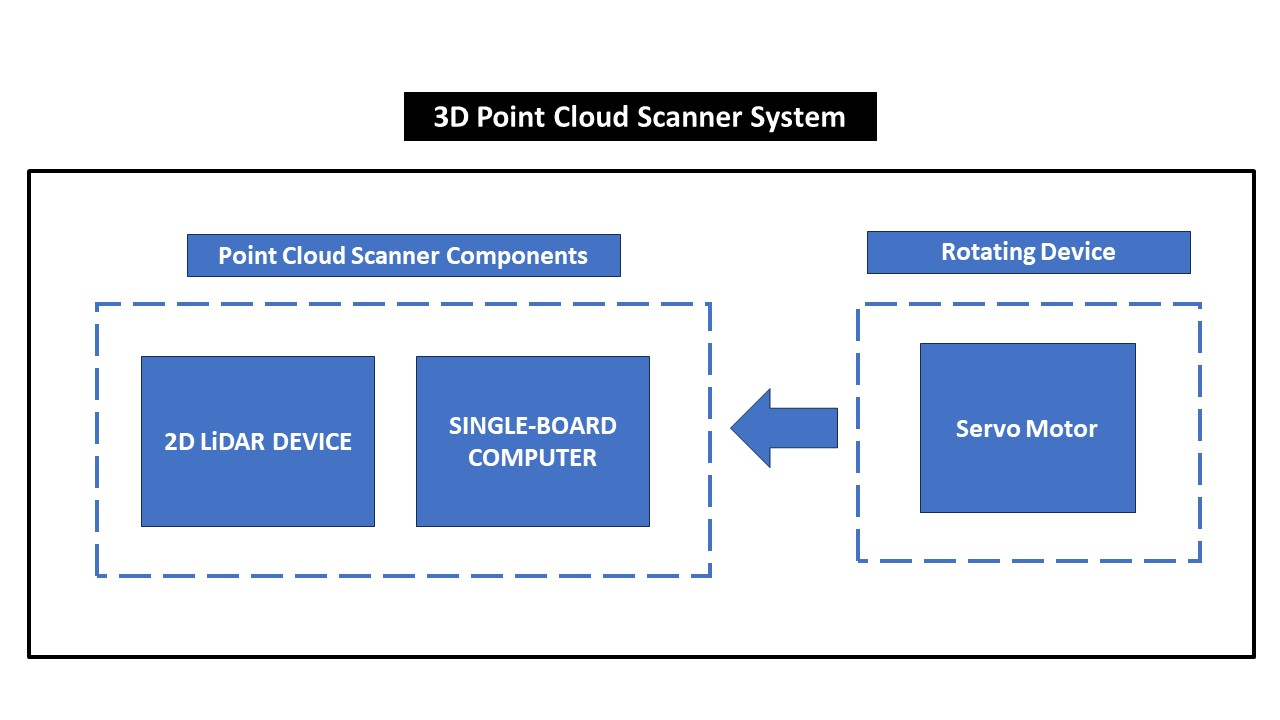
\includegraphics[width=1\textwidth]{Figures/3D-PCSS components}
	\caption{Major Components of 3D-PCSS}
	\label{ch4:fig:components_of_3d-pcss}
\end{figure}

\begin{figure}[H]
	\centering
	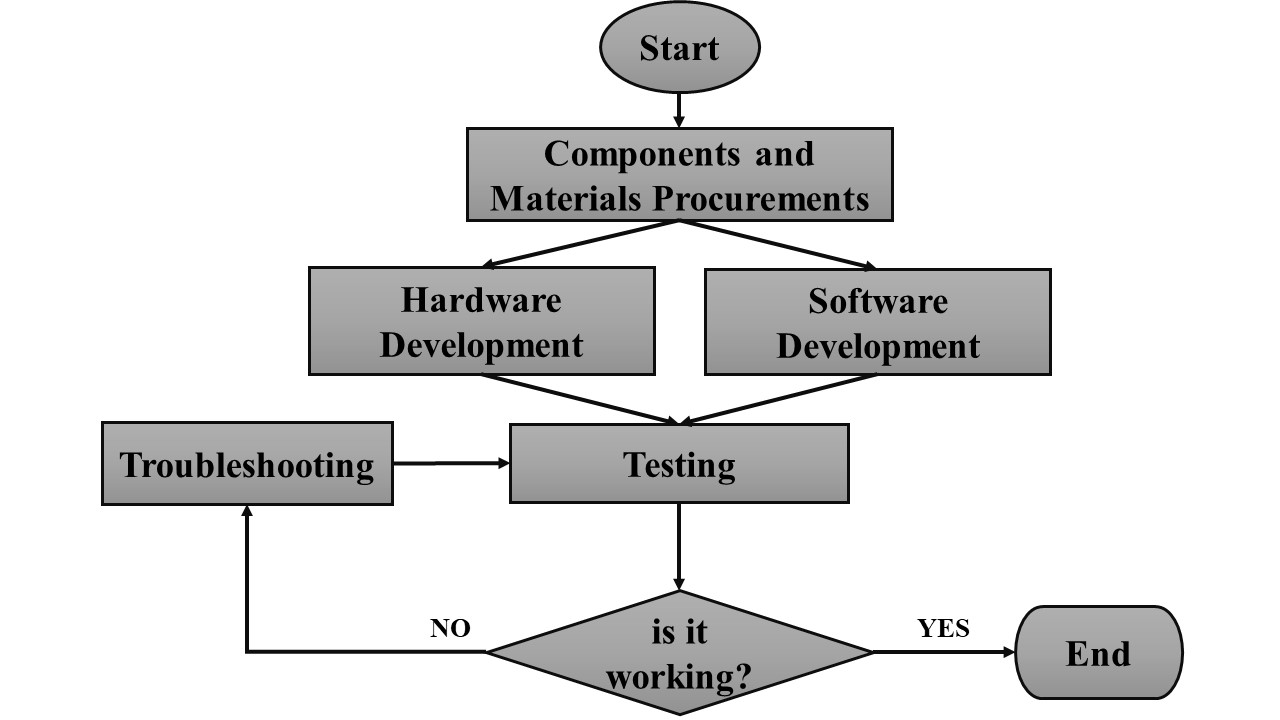
\includegraphics[width=0.8\textwidth]{Figures/hardware_flowchart}
	\caption{Hardware Design Flow Chart}
	\label{ch4:fig:3d-pcss_development_flow_chart}
\end{figure}

% \subsection{Data Gathering}
% For the data gathering of the raw point cloud, all the major hardware of the system will be assemble and integrate as shown in Figure \ref{ch4:fig:System Hardware Block Diagram}. The scanned data from the 2D LiDAR sensor will be received by small computer which is Raspberry Pi for the processing of the raw data. This small computer is connected to the internet in order to control remotely by the personal laptop. Different scanning procedure will be performed to gather point cloud data.

% \begin{figure}[H]
% 	\centering
% 	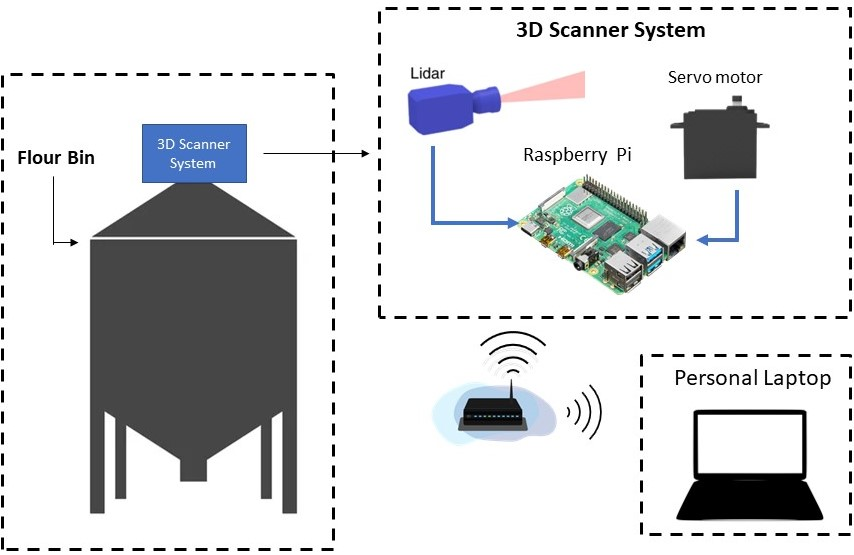
\includegraphics[width=0.9\textwidth]{Figures/system-hardware-block-diagram.jpg}
% 	\caption{System Hardware Block Diagram}
% 	\label{ch4:fig:System Hardware Block Diagram}
% \end{figure}

\section{Software Development}
\label{ch4:sec:firmware_development_design}

Software design plays a crucial role in the development of the 3D-PCSS by facilitating communication between hardware components, and allows connection with external software system. The system was designed to initialize all necessary components, including nodes and connection, immediately upon power-up. This ensures seamless operation and also establish connection with the developed web application for user interaction. As described in figure \ref{ch4:fig:software_system_process}, after turning on the system, it initializes essential nodes and enter in idle mode waiting for an external command coming from the web application. The system remain in idle mode unless turnoff. The development of software processes, including the choice of operating system and frameworks is outlined in this section.

Throughout this study, it's important to note that the terms 'process' and 'nodes' are used interchangeably. This interchangeable usage highlights the fundamental concept in ROS where processes, represented as nodes, perform computation and communication tasks within the system.

\begin{figure}[H]
	\centering
	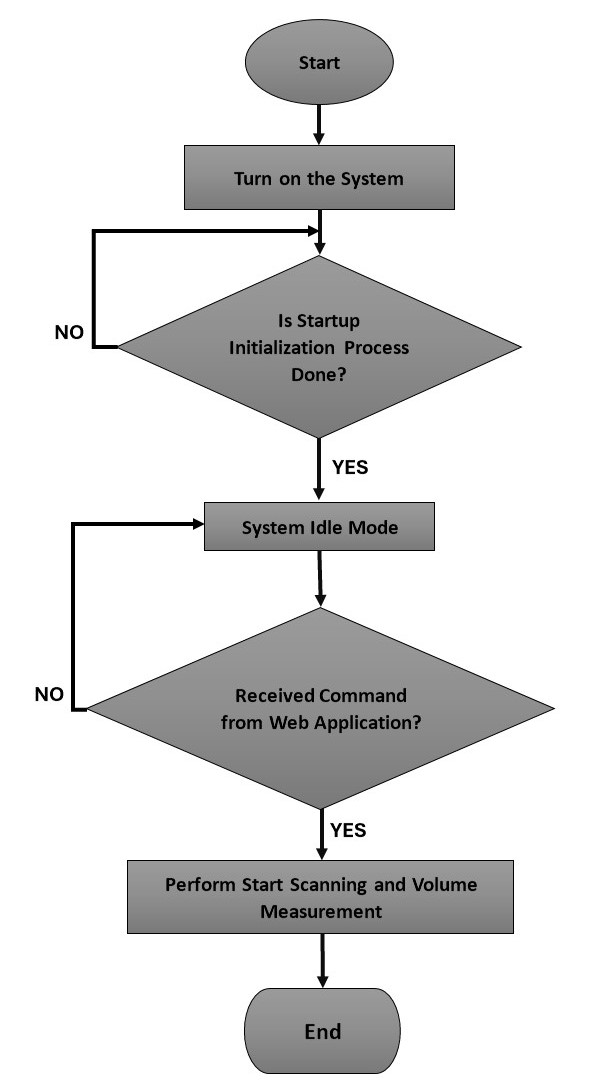
\includegraphics[width=0.7\textwidth, height=0.7\textheight]{Figures/software_system_process}
	\caption{System Process Flow Chart}
	\label{ch4:fig:software_system_process}
\end{figure}

\subsection{Operating System and Frameworks}

In this study, the single-board computer (SBC) used in the 3D-PCSS requires an appropriate OS and frameworks to support the execution of firmware and software components. Linux-based operating systems, such as Ubuntu, is commonly chosen for SBCs due to its reliability, flexibility, and extensive community support. This OS option provide a stable platform for running Robot Operating System (ROS) nodes and managing system resources effectively, thus, was utilized in this study. ROS framework was also utilized in this study to develop a publish-subscribe relationship between ROS nodes. Lastly, Point Cloud Library (PCL) serves in this study as a fundamental library being used for processing and analyzing point cloud data. PCL provides a comprehensive set of algorithms and tools for tasks such as point cloud registration, filtering and computational geometry to name a few.

\subsection{Startup Initialization Process}
Roscore and rosgridge are the two essential cores that used in the 3D-PCSS. These cores or nodes typically need to be manually started in the command-line interface (CLI) or desktop environment to run and process data, or to initiate other nodes and do specific tasks. In this study, a custom service file was developed to automate and start these nodes after the system is turnon. This file is created using Linux systemd to configure and instantly run the necessary programs or nodes.

% The Raspberry Pi will receive the scanned raw data coming from the 3D point cloud scanner. This data will be processed in different stages to produced desired output, such as point cloud pre-processing (formatting, converting, clustering, and cleansing) and post-processing (e.g., 3D mapping and volume measurement). Various platforms and frameworks nowadays are available to ease the handling of these massive raw data, thus, formatting the data to a desired platform must be perform. Typically, the value of raw data coming from the LiDAR sensor is not directly a point cloud data but rather a value of the distance between the sensor and the reflected nearest object in a particular direction, therefore, the data is converted into point cloud which composed of x, y, and z values. The Equation \eqref{ch4:eq:x-point}, \eqref{ch4:eq:y-point}, and \eqref{ch4:eq:z-point} is conversion of polar coordinates (distance, angle) to cartesian coordinates x, y, and z, respectively, in a 3D coordinate system.

% \begin{equation}
% 	x_{point_{i}} = \ \sin(i) \times d \
% 	\label{ch4:eq:x-point}
% \end{equation}
% \begin{equation}
% 	y_{point_{i}} = \ \cos(\pi) \times \cos(i) \times d \
% 	\label{ch4:eq:y-point}
% \end{equation}
% \begin{equation}
% 	z_{point_{i}} = \ -\cos(i) \times \sin(\pi) \times d \
% 	\label{ch4:eq:z-point}
% \end{equation}

% Where:

% \indent \indent i = scan angle of the scanner

% \indent \indent d = the distance point of the emitted pulse by the LiDAR (meter)

\subsection{System Scanning and Point Cloud Processes}

The researcher will create an algorithm for clustering and cleansing of the raw data. The data will be clustered into two parts, the outliers (dust) data and the inliers (target) data. Based on the behaviors and characteristics of dust, the researcher will use the Multi-echo method for outlier clustering because the laser emitted by the LiDAR will penetrate through the dust cloud and will receive multiple return. Another method that the researcher will utilize is the low-intensity method clustering for outliers due to the characteristic of the dust having a lower intensity compared to other objects. The data cleansing will be employed after all the data is being clustered. After of these processes, the researcher will convert the pre-processed point cloud for further analysis.

\subsection{Volume Estimation}
\label{ch4:sec:Volume Estimation}
The researcher will create an algorithm for volume estimation of the material inside the flour bin using Delaunay Triangulation which creates a mesh of triangles such that no point is inside the the circumference of any of the triangle. Convex Hull is a subset of Delaunay Triangulation which creates a boundary on the same given points, all the triangles are on the boundary of the point set. The computation of the estimated volume of the material inside the bin is shown in Figure \ref{ch4:fig:volume-estimation-figure} and Equation \eqref{ch4:eq:volume-estimation}.

\begin{figure}[H]
	\centering
	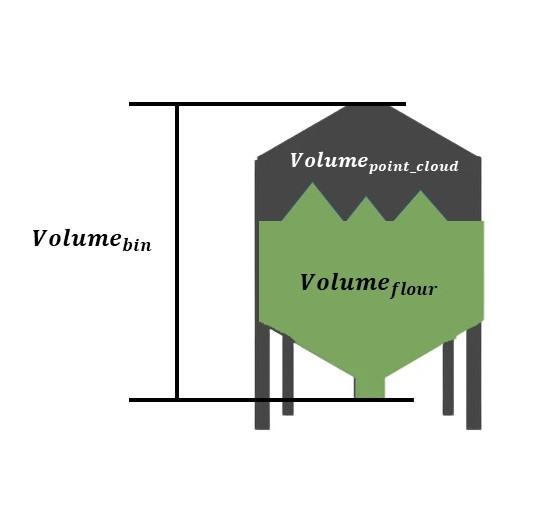
\includegraphics[width=0.8\textwidth]{Figures/volume-estimation-figure}
	\caption{Volume of the flour is the difference between the volume of the bin and volume of the point cloud}
	\label{ch4:fig:volume-estimation-figure}
\end{figure}

\begin{equation}
	Volume_{flour} = Volume_{bin} - Volume_{point\_cloud}
	\label{ch4:eq:volume-estimation}
\end{equation}

\section{Web-based Application Development}
This custom user interface based on web application is developed to used for the 3D-PCSS. The tools, framework and and resources of the system is discussed in this section.

The user interface consider the following design and functionality, the UI should be:
\begin{itemize}
	\item Intuitive and simple.
	\item Able to establish connection to the 3D-PCSS.
	\item Able to send command, display 3D point cloud data and volume measurement.
\end{itemize}

\section{Overall System Testing and Evaluation}
\label{ch4:sec:Testing and Evaluation}
In this section, Different testing was conducted

\subsection{Different Testing Procedure}
\label{ch4:subsec:Different Testing Procedure}
The researcher will conduct different testing and evaluation to observe the accuracy of the system. In the experiment, the researcher will ensure that the prototype flour bin is scanned remotely and without any human intervention. The researcher intends to perform multiple tests to assess the filtering method and validate the precision and effectiveness of the object's volume measurement, and each of the testing will have a multiple trials. The different testing procedure of the system are the following:
\begin{enumerate}
	\item \label{ch4:first} The system will scan the created different shape of flour bin without materials and dust inside.
	\item \label{ch4:second} The researcher will generate a dust in the flour bin but without material inside and scan the bin.
	\item \label{ch4:third} The searcher will scan the flour bin with flour material inside with different surface shape but without dust.
	\item \label{ch4:fourth} The researcher will generate dust from the testing structure conducted in testing \ref{ch4:third}
\end{enumerate}

\subsection{Evaluation of the System}
\label{ch4:subsec:Evaluation of the System}
Based on the conducted different testing mentioned in \ref{ch4:subsec:Different Testing Procedure}, the researcher will evaluate the conducted testing based on the volume of scanned data. System in the following evaluation

To evaluate the testing \ref{ch4:first}, the researcher will measure the accuracy of the system by comparing the estimated volume of the system  with the actual volume of the different shape of the bin, calculate the error percentage for each trial and assess the over all precision of the system. Table \ref{ch4:tab:Testing 1} shows the sample comparison of the testing.

\begin{table}[H]
	\caption{Testing \ref{ch4:first}}
	\label{ch4:tab:Testing 1}
	\centering
	\begin{tabular}{|c|c|c|c|}
		\hline
		% First row
		Flour bin Shape & Actual Volume (\si{mm^3}) & Scanned Volume (\si{mm^3}) & Error (\%) \\
		\hline
		\multicolumn{4}{|c|}{Trial 1}                                                         \\
		\hline
		% Second row
		Cube            & -                         & -                          & -          \\
		\hline
		% Third row
		Cylinder        & -                         & -                          & -          \\
		\hline
		\multicolumn{4}{|c|}{Trial 2}                                                         \\
		\hline
		Cube            & -                         & -                          & -          \\
		\hline
		% Third row
		Cylinder        & -                         & -                          & -          \\
		\hline
	\end{tabular}
\end{table}

Testing \ref{ch4:second} will be evaluated from the testing \ref{ch4:first} based on the number of point cloud acquired of both testing, and compare it. Basically, the testing \ref{ch4:second} will acquired more point cloud compared to testing \ref{ch4:first} due to multi-echo or multiple returning from the dust and the flour bin.

In testing \ref{ch4:third} and \ref{ch4:fourth}, the researcher will place flour materials inside the bin with different surface shape and perform volume estimation. After the volume estimation, the researcher will generate dust, scan the bin, perform volume estimation and compare it to the result of the testing \ref{ch4:third}. The sample result of testing \ref{ch4:third} and \ref{ch4:fourth} is shown in table

\begin{table}[H]
	\caption{Testing 3 and 4}
	\label{ch4:tab:Testing 3 and 4}
	\centering
	\begin{tabular}{|c|p{0.27\linewidth}|p{0.26\linewidth}|p{0.2\linewidth}|}
		\hline
		% First row
		Flour bin Shape & Scanned Volume (without dust) & Scanned Volume (with dust) & Error (\%) \\
		\hline
		\multicolumn{4}{|c|}{Surface Shape 1}                                                     \\
		\hline
		% Second row
		Cube            & -                             & -                          & -          \\
		\hline
		% Third row
		Cylinder        & -                             & -                          & -          \\
		\hline
		\multicolumn{4}{|c|}{Surface Shape 2}                                                     \\
		\hline
		Cube            & -                             & -                          & -          \\
		\hline
		% Third row
		Cylinder        & -                             & -                          & -          \\
		\hline
	\end{tabular}
\end{table}